\chapter{XÂY DỰNG VÀ KIỂM THỬ HỆ THỐNG}

\section{Xây dựng Giao diện người dùng (UI)}
Giao diện của hệ thống được xây dựng hoàn toàn bằng Next.js (App Router) và Tailwind CSS, mang lại trải nghiệm mượt mà, phản hồi siêu tốc. Toàn bộ giao diện sử dụng thiết kế Responsive, tương thích trên cả Desktop và Mobile.

\subsection{Cấu trúc thư mục Frontend}
Mã nguồn Frontend được tổ chức theo kiến trúc App Router của Next.js:

\begin{verbatim}
frontend/src/
|-- app/
|   |-- (public)/          # 10 trang cong khai
|   |   |-- page.tsx       # Trang chu (SSR)
|   |   |-- bang-gia/      # Bang gia + QR
|   |   |-- tin-tuc/       # Tin tuc + [slug]
|   |   |-- dich-vu/       # Dich vu + [slug]
|   |   |-- lien-he/       # Form lien he -> API
|   |   |-- doi-tac/       # Form affiliate -> API
|   |   |-- Header.tsx     # Navbar + Hamburger
|   |   \-- Footer.tsx     # Footer
|   |-- admin/             # 8 trang quan tri
|   |   |-- dashboard/     # Thong ke tong quan
|   |   |-- services/      # CRUD goi dich vu
|   |   |-- news/          # CRUD tin tuc
|   |   |-- orders/        # Quan ly don hang
|   |   |-- promotions/    # CRUD khuyen mai
|   |   \-- audit-logs/    # Nhat ky he thong
|   \-- layout.tsx         # Root layout + SEO
|-- lib/axios.ts           # apiClient cau hinh
|-- middleware.ts          # Auth middleware
\-- types/index.ts         # TypeScript interfaces
\end{verbatim}

\subsection{Giao diện Landing Page công khai}
Trang Landing Page tập trung vào việc hiển thị các thông tin giới thiệu, các lợi thế cạnh tranh (như cam kết Uptime 99.99\%) và bảng giá dịch vụ để thu hút người mua.

Các trang công khai chính gồm: Trang chủ, Giới thiệu, Dịch vụ (danh sách + chi tiết theo slug), Bảng giá (toggle Tháng/Năm + mã QR), Khách hàng (testimonials), Tin tức (danh sách + chi tiết), Liên hệ (form gửi API) và Đối tác (form đăng ký affiliate).

% TODO: Chèn ảnh giao diện trang chủ. Hãy lưu file ảnh tên là 'landing_home.png' vào thư mục 'images'
\begin{figure}[htbp]
    \centering
    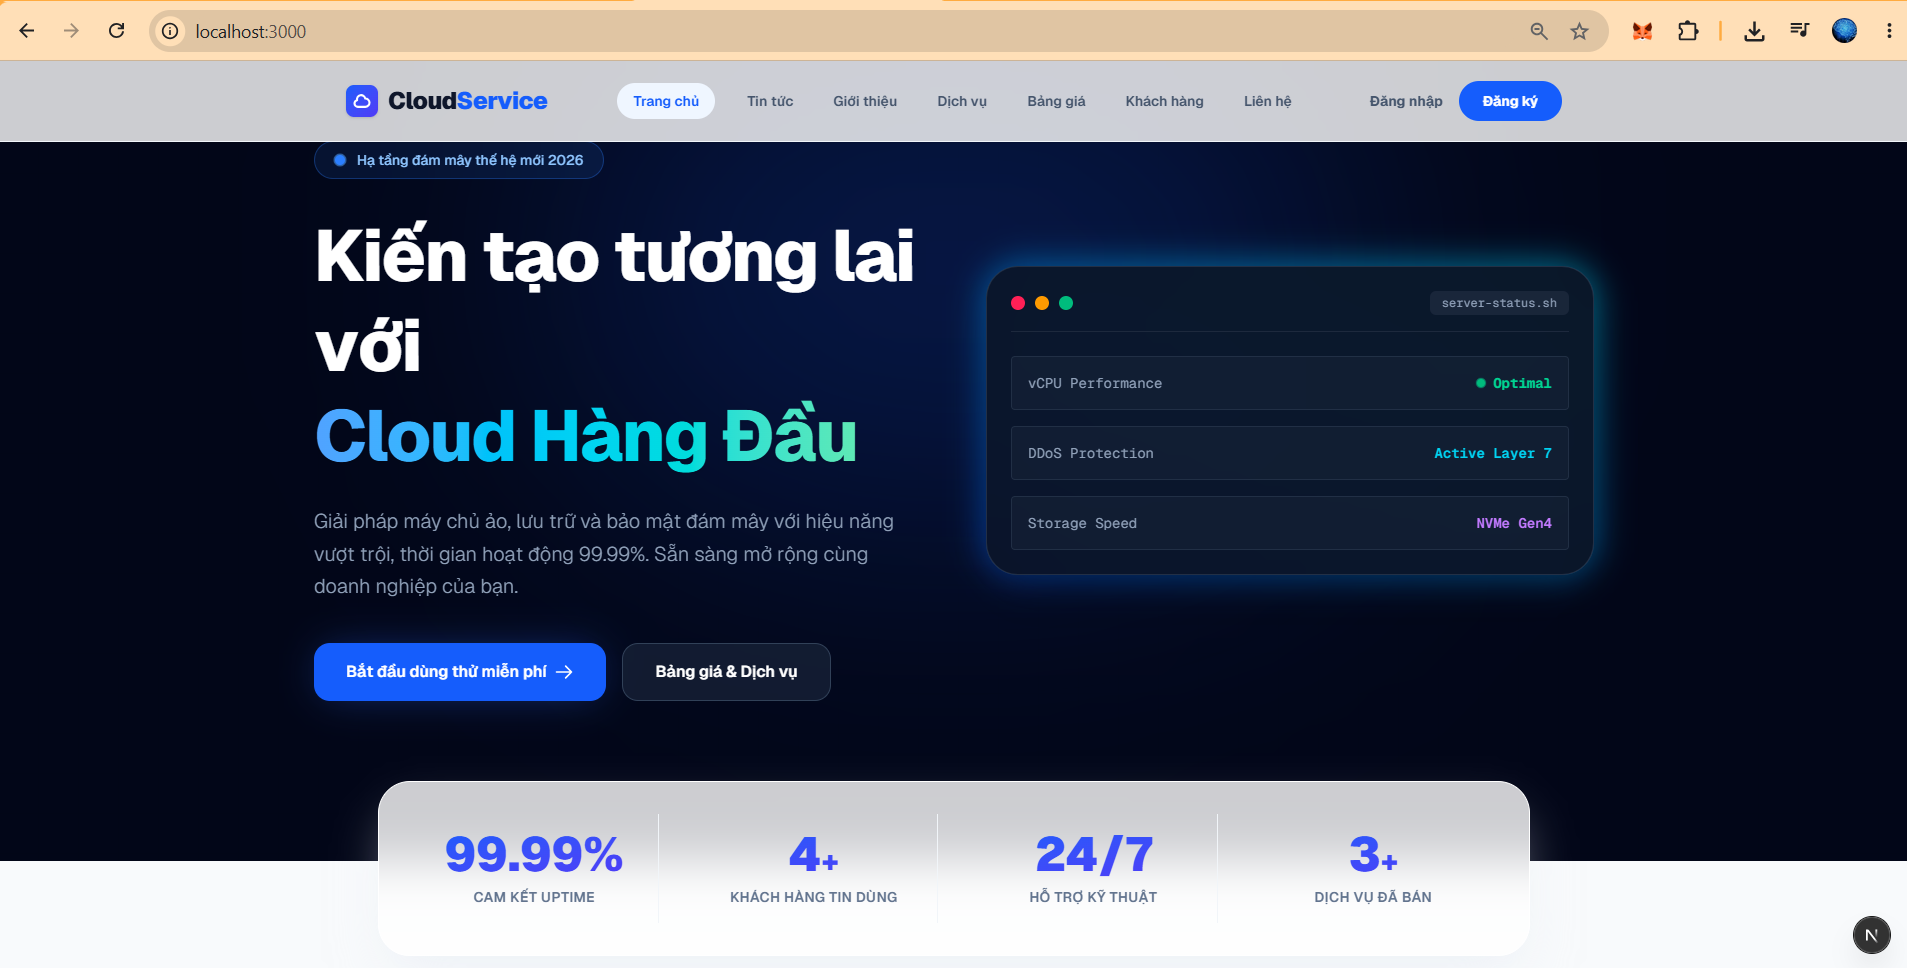
\includegraphics[width=0.9\textwidth]{images/landing_home.png}
    \caption{Giao diện trang chủ (Landing Page)}
    \label{fig:landing_home}
\end{figure}

% TODO: Chèn ảnh giao diện trang Bảng giá. Hãy lưu file ảnh tên là 'landing_pricing.png' vào thư mục 'images'
\begin{figure}[htbp]
    \centering
    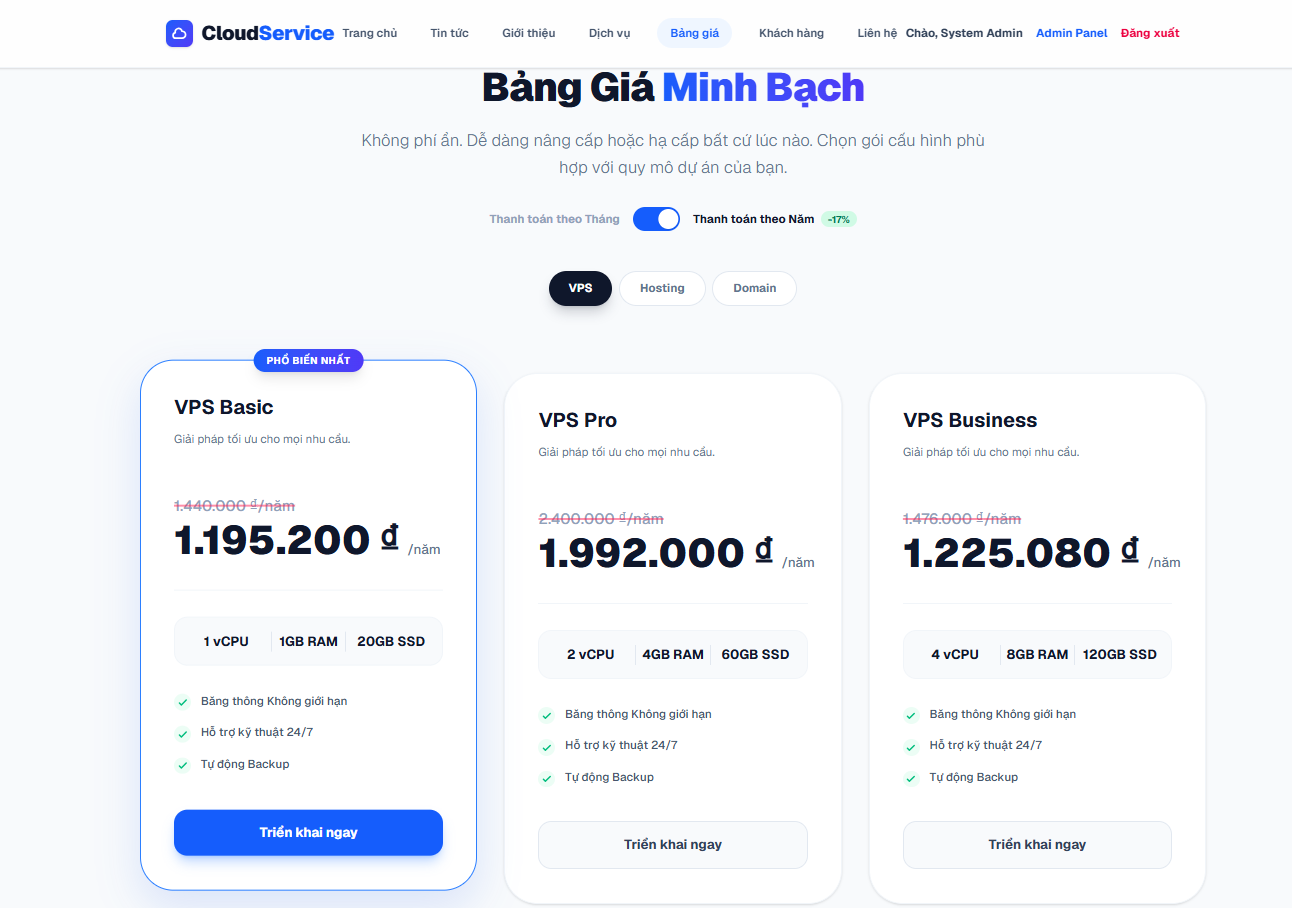
\includegraphics[width=0.9\textwidth]{images/landing_pricing.png}
    \caption{Giao diện trang Bảng giá -- Chuyển đổi Tháng/Năm và hiển thị mã QR}
    \label{fig:landing_pricing}
\end{figure}

\subsection{Giao diện Quản trị (Admin Dashboard)}
Sau khi xác thực thành công qua JWT tại trang \texttt{/login}, hệ thống dựa vào Role của người dùng để điều hướng đến Admin Dashboard. Giao diện quản trị bao gồm sidebar navigation cố định bên trái và khu vực nội dung chính bên phải.

Các trang Admin chính bao gồm:
\begin{itemize}
    \item \textbf{Dashboard:} Hiển thị thống kê tổng quan (tổng đơn hàng, doanh thu, số bài viết) qua các thẻ card và biểu đồ doanh thu theo tháng, dữ liệu lấy từ API \texttt{/admin/stats/summary} và \texttt{/admin/stats/revenue-chart}.
    \item \textbf{Quản lý Tin tức:} Hỗ trợ CRUD đầy đủ (Thêm/Sửa/Xóa bài viết) qua modal form, dữ liệu đồng bộ real-time với Backend.
    \item \textbf{Quản lý Đơn hàng:} Hiển thị danh sách đơn hàng, cho phép thay đổi trạng thái (Pending $\rightarrow$ Processing $\rightarrow$ Completed/Rejected) và xuất ra file Excel.
    \item \textbf{Quản lý Khuyến mãi:} Tạo và xóa chương trình khuyến mãi (mã code, phần trăm giảm, thời hạn).
    \item \textbf{Audit Logs:} Xem lịch sử hành động của hệ thống (ai đăng nhập, từ IP nào, lúc mấy giờ).
\end{itemize}

% TODO: Chèn ảnh giao diện Admin Dashboard. Hãy lưu file ảnh tên là 'dashboard_admin.png' vào thư mục 'images'
\begin{figure}[htbp]
    \centering
    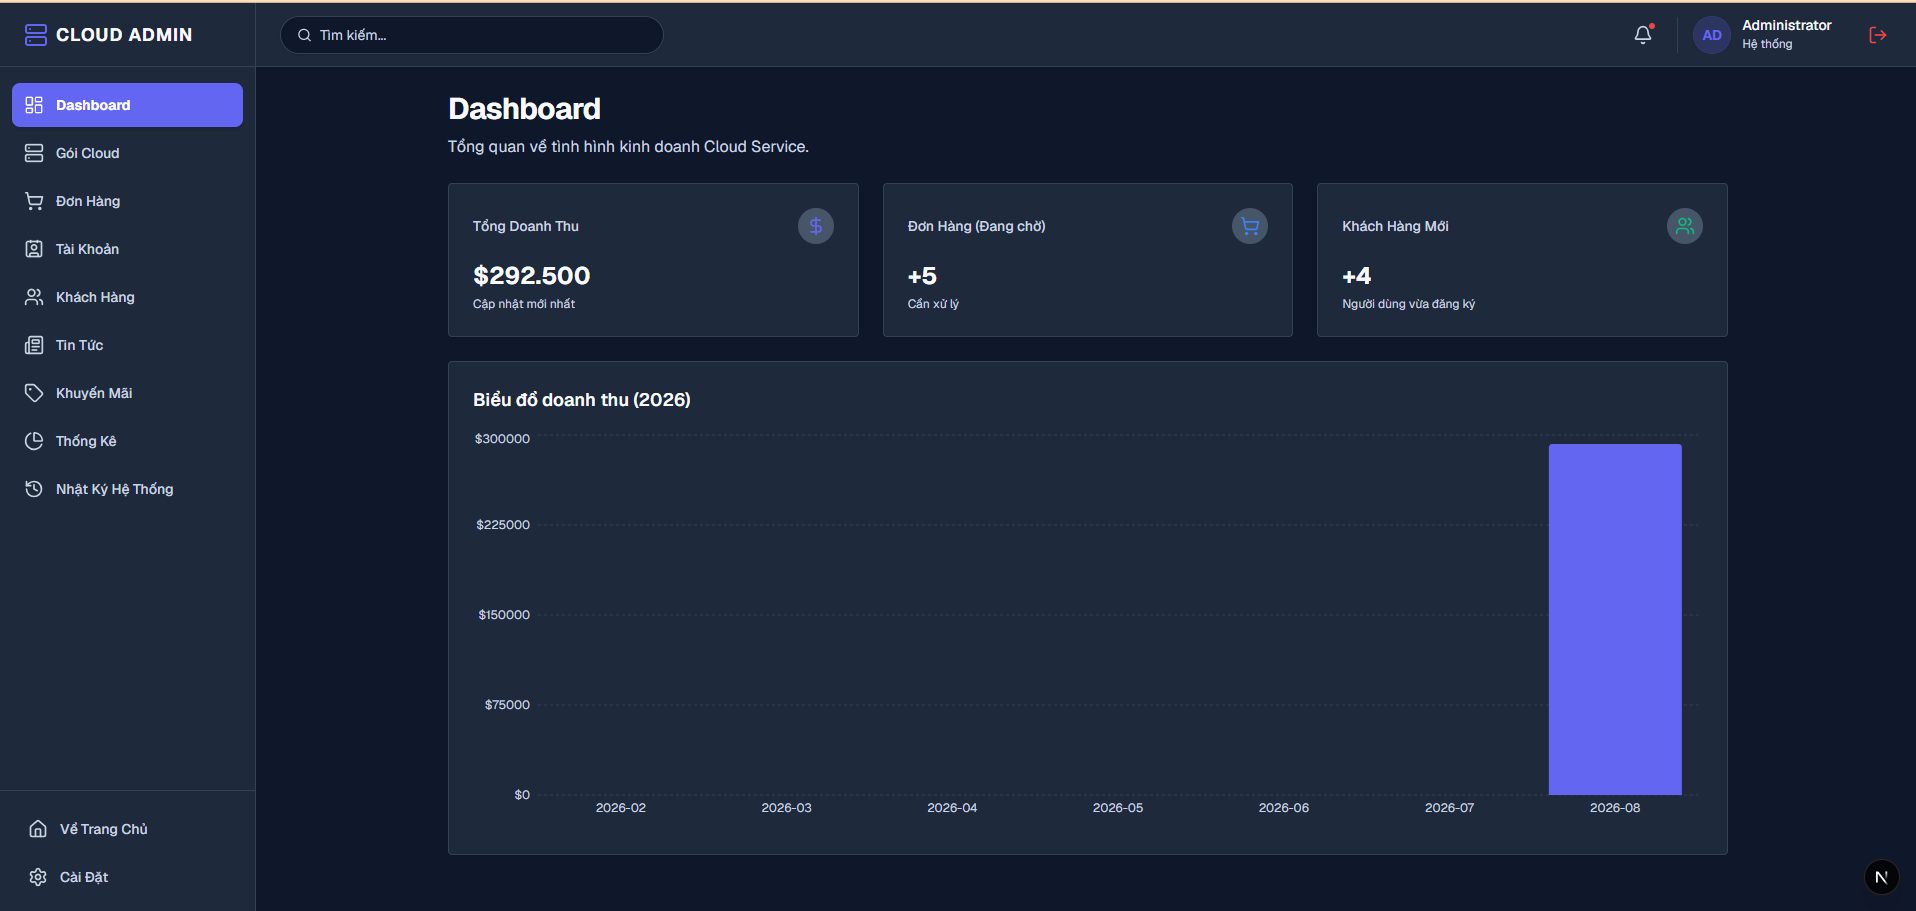
\includegraphics[width=0.9\textwidth]{images/dashboard_admin.png}
    \caption{Giao diện Bảng điều khiển Quản trị viên (Admin Dashboard)}
    \label{fig:dashboard_admin}
\end{figure}

\section{Kiểm thử đơn vị (Unit Testing)}
Kiểm thử phần mềm là một khâu không thể thiếu để đảm bảo độ tin cậy của sản phẩm. Dự án đã viết mã kiểm thử tự động sử dụng framework \textbf{xUnit} và thư viện mock \textbf{Moq} trên .NET trong project riêng biệt \texttt{CloudService.UnitTests}.

\subsection{Tổng quan kết quả}
Tổng cộng \textbf{16 test cases} (vượt yêu cầu tối thiểu 15) đã được viết và chạy thành công, phân bổ theo 5 file test:

\begin{table}[htbp]
    \centering
    \caption{Chi tiết kết quả Unit Test}
    \label{tab:unit_tests}
    \begin{tabular}{|c|p{5cm}|c|p{5cm}|}
        \hline
        \textbf{STT} & \textbf{File Test} & \textbf{Số test} & \textbf{Đối tượng kiểm thử} \\
        \hline
        1 & \texttt{OrderServiceTests.cs} & 6 & Tạo đơn hàng, đổi trạng thái, validate input, lấy danh sách, xử lý lỗi \\
        \hline
        2 & \texttt{ServicePlanServiceTests.cs} & 5 & CRUD gói dịch vụ, tính giá theo chu kỳ, validate specs \\
        \hline
        3 & \texttt{AffiliateServiceTests.cs} & 2 & Tạo đơn đăng ký affiliate, đổi trạng thái \\
        \hline
        4 & \texttt{CategoryServiceTests.cs} & 2 & CRUD danh mục, kiểm tra trùng tên \\
        \hline
        5 & \texttt{NewsArticleServiceTests.cs} & 1 & Tạo bài viết mới, generate slug \\
        \hline
        \multicolumn{2}{|c|}{\textbf{Tổng cộng}} & \textbf{16} & Tất cả PASSED \\
        \hline
    \end{tabular}
\end{table}

\subsection{Phương pháp Mock}
Mỗi test case sử dụng thư viện \textbf{Moq} để tạo đối tượng giả lập (mock) cho các Repository và UnitOfWork, giúp cô lập logic nghiệp vụ tại tầng Application mà không cần kết nối đến cơ sở dữ liệu thực. Ví dụ trích code test:

\begin{verbatim}
[Fact]
public async Task CreateOrder_WithValidData_ReturnsSuccess()
{
    // Arrange - Tạo mock repository
    var mockRepo = new Mock<IOrderRequestRepository>();
    var mockUoW = new Mock<IUnitOfWork>();
    mockUoW.Setup(u => u.Orders).Returns(mockRepo.Object);

    var service = new OrderService(mockUoW.Object);
    var dto = new CreateOrderDto {
        CustomerName = "Nguyen Van A",
        Email = "test@email.com",
        ServiceName = "VPS Pro"
    };

    // Act - Gọi hàm cần test
    var result = await service.CreateAsync(dto);

    // Assert - Kiểm tra kết quả
    Assert.NotNull(result);
    mockUoW.Verify(u => u.CompleteAsync(), Times.Once);
}
\end{verbatim}

% TODO: Chèn ảnh kết quả chạy Test. Hãy lưu file ảnh tên là 'unit_test_result.png' vào thư mục 'images'
\begin{figure}[htbp]
    \centering
    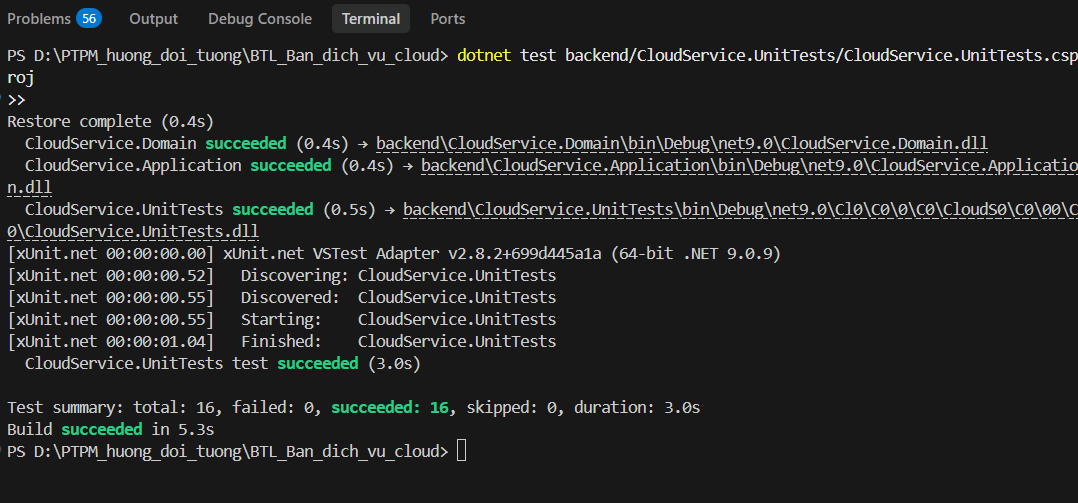
\includegraphics[width=0.8\textwidth]{images/unit_test_result.png}
    \caption{Kết quả chạy 16 Unit Test toàn bộ PASSED}
    \label{fig:unit_test_result}
\end{figure}

\section{Triển khai liên tục (CI/CD) và Docker}
Dự án áp dụng quy trình Phát triển phần mềm hiện đại, tuân thủ nguyên tắc ``Cộng tác chặt chẽ''. Mã nguồn được quản lý phiên bản qua Git trên GitHub.

\subsection{Luồng làm việc với GitHub Actions (CI)}
Mọi thao tác đẩy mã (Push) lên nhánh \texttt{develop} hoặc \texttt{main}, và mọi Pull Request đều kích hoạt pipeline GitHub Actions. Nội dung pipeline \texttt{.github/workflows/ci.yml}:

\begin{enumerate}
    \item \textbf{Checkout:} Kéo mã nguồn từ repository.
    \item \textbf{Setup .NET 9:} Cài đặt môi trường .NET SDK phiên bản 9.0.x.
    \item \textbf{Restore:} Khôi phục thư viện NuGet cho cả API và Unit Test project.
    \item \textbf{Build:} Biên dịch mã nguồn ở chế độ Release.
    \item \textbf{Test:} Chạy toàn bộ 16 Unit Tests. Nếu bất kỳ test nào thất bại, pipeline sẽ báo Failed và không cho phép merge PR.
\end{enumerate}

\subsection{Đóng gói ứng dụng với Docker}
Để giải quyết bài toán ``Chạy được trên máy tôi nhưng lỗi trên máy chủ'', toàn bộ hệ thống được cấu hình vào các Container riêng biệt:

\begin{itemize}
    \item \textbf{Dockerfile (Backend):} Multi-stage build: stage 1 (build) sử dụng image \texttt{dotnet/sdk:9.0} để biên dịch, stage 2 (runtime) sử dụng image \texttt{dotnet/aspnet:9.0} gọn nhẹ để chạy.
    \item \textbf{docker-compose.yml:} Định nghĩa 2 services:
    \begin{itemize}
        \item \texttt{sqldb}: SQL Server 2022 Express với dữ liệu lưu trên volume \texttt{sql\_data}.
        \item \texttt{backend}: API .NET 9 kết nối tới container \texttt{sqldb}, expose port 5000.
    \end{itemize}
\end{itemize}

Chỉ với một dòng lệnh duy nhất \texttt{docker compose up -d}, hệ thống đã được triển khai sẵn sàng trên mọi hệ điều hành hoặc máy chủ Cloud thực tế.

\subsection{Quy trình làm việc nhóm với Git}
Nhóm áp dụng mô hình \textbf{Feature Branch Workflow}:
\begin{enumerate}
    \item Mỗi tính năng được phát triển trên một nhánh riêng (ví dụ: \texttt{feature/admin-dashboard}).
    \item Khi hoàn thành, tạo Pull Request (PR) lên nhánh \texttt{develop}.
    \item Các thành viên khác review code và approve.
    \item CI pipeline tự động chạy build + test. Nếu PASSED, PR được phép merge.
    \item Nhánh \texttt{main} chỉ chứa code ổn định, sẵn sàng triển khai.
\end{enumerate}
